\chapter{Grafický komponent v Inkscape}

\section{Vytvorenie SVG v programe Inkscape}

Nakreslenie jednotlivých častí komponentov prečerpávacej stanice bolo realizované pomocou ľavého bočného panela. Prečerpávacia stanica sa skladá z rúriek, ventila, nádrže, hladiny vody, motora, vrtuliek. Ako je možné vidieť na obrázku \ref{picture1}.  

\begin{figure}[ht]
	\begin{center}
		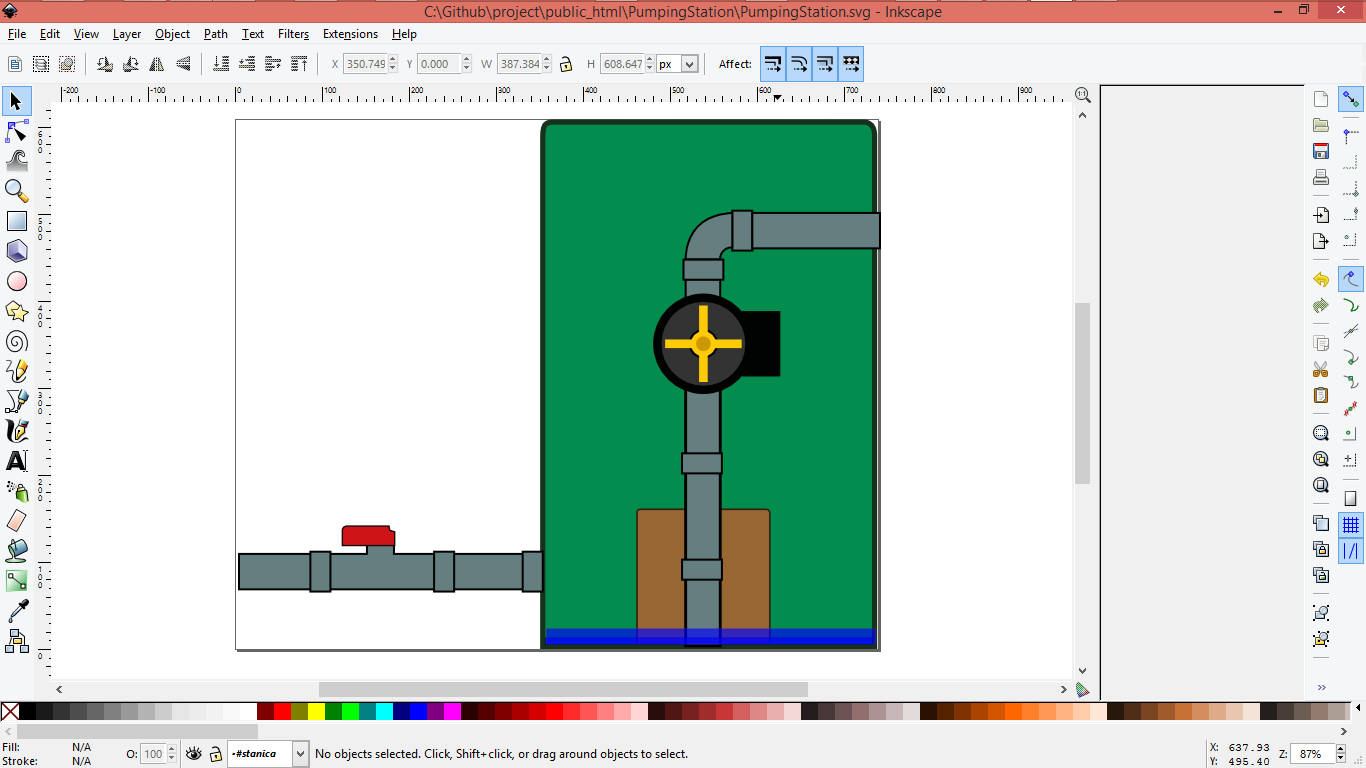
\includegraphics [width=15cm] {obrazky/obr1.png}
		\caption{Grafické prostredie programu Inkscape s nakreslenou prečerpávacou stanicou}
		\label{picture1}
	\end{center}
\end{figure}


\section{Zistenie id SVG}

Pre ovládanie JavaScriptom je nutné si pozrieť jednotlivé jedinečné identifikačné názvy. Sú v SVG označované ako id. Zistenie id je pomerne jednoduché. Klikneme pravým tlačidlom na daný komponent, ktorého id chceme vedieť, a potom na Objekt Properties. Ako je možné vidieť na obrázku \ref{picture2}.

\begin{figure}[ht]
	\begin{center}
		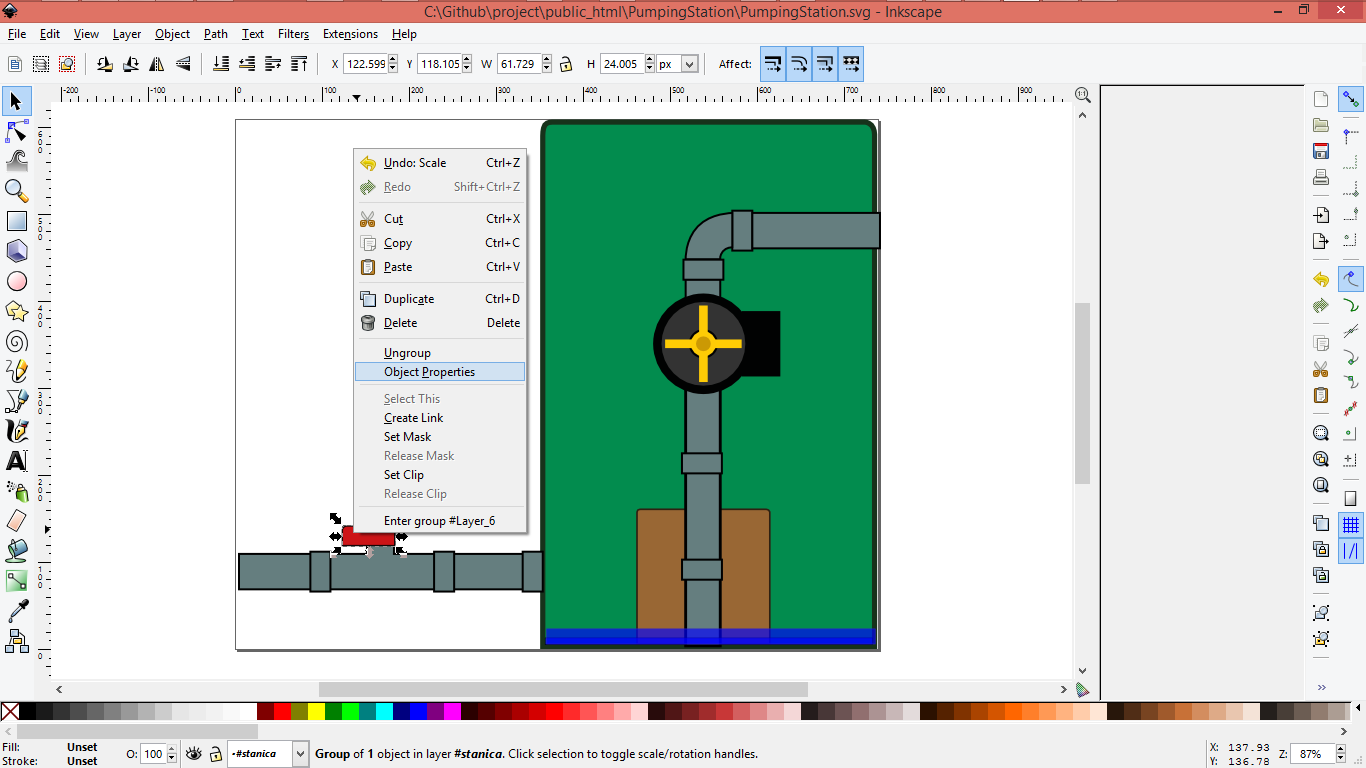
\includegraphics [width=15cm] {obrazky/obr2.png}
		\caption{Zobrazenie menu pre daný objekt v Inkscape}
		\label{picture2}
	\end{center}
\end{figure}

Po stlačení sa nám zobrazí nasledovné okno viď obrázok \ref{picture3}. 

\begin{figure}[ht]
	\begin{center}
		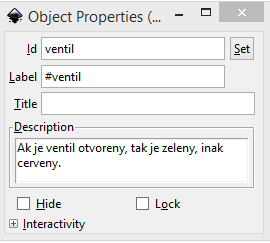
\includegraphics  {obrazky/obr3.png}
		\caption{obrázok 3}
		\label{picture3}
	\end{center}
\end{figure}


Z obrázka možno vyčítať aké je ID, predvolené sú tam napr. desc3072. Hodnoty je možné prepísať a zmeniť stlačením tlačidla Set. Pre nás je dôležitá hodnota v kolónke Label - \#ventil. Toto nám umožni potom neskôr ako CSS selektor, cez ktorý budeme môcť ovládať danú časť. Spravidla hodnoty ID a Label sú rovnaké. Líšia sa iba v tom, že pri Label je pridaný znak \# pred názvom. ID je unikátny názov pre program Inkscape. 

Alebo ďalší spôsob zistenia id SVG časti tvarov je priamo nájsť tú hodnotu v PumpingStation.svg. Je to označené ako id="ventil".

V okne Object Properties je možné nastaviť script na animovanie. Po kliknutí na Interactivity sa zobrazia ďalšie kolónky, kde je možné zadať akciu, ktorá má nastať.  

%\begin{figure}[ht]
%	\begin{center}
%		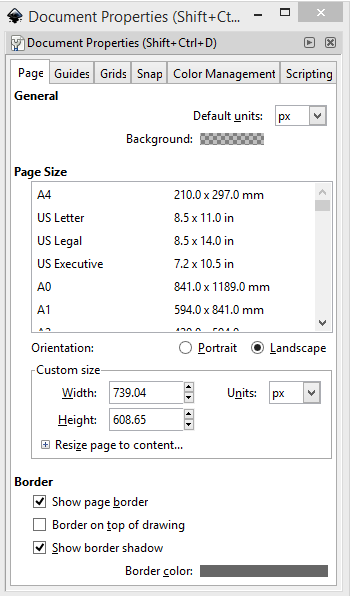
\includegraphics[height=7cm]  {obrazky/obr4.png}
%		\caption{obrázok 4}
%		\label{picture4}
%	\end{center}
%\end{figure}


\subsection{XML Editor}
Ďalší spôsob získania informácii o svg cez Inkscape je cez zabudovaný XML Editor.
Stlačením klávesovej skratky SHIFT + CTRL + X, alebo v hornej lište v menu vybrať ponuku Edit a na spodu je XML Editor. Následne sa zobrazí okno, ktoré je na obrázku \ref{xmlEditor}.
\begin{figure}[ht]
	\begin{center}
		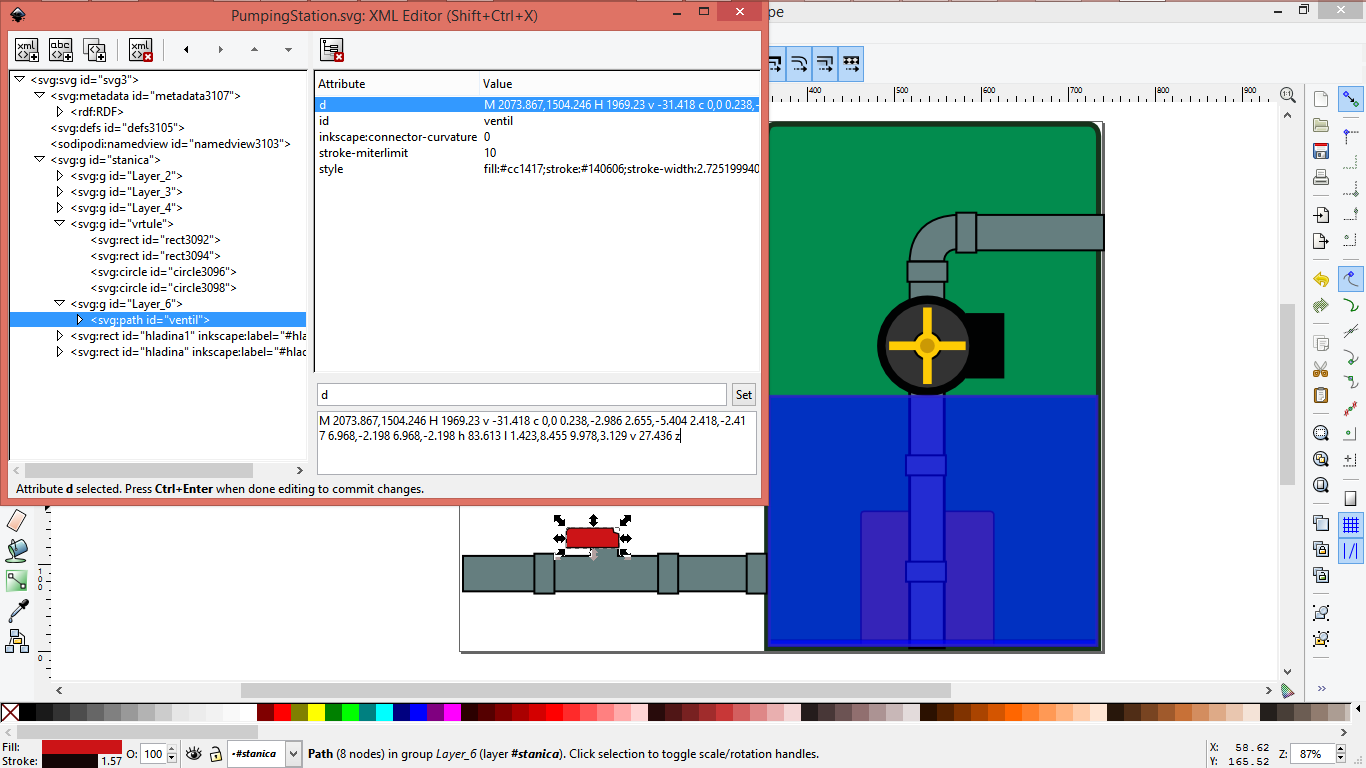
\includegraphics[width=10cm]  {obrazky/XmlEditor.png}
		\caption{Xml Editor v Inkscape}
		\label{xmlEditor}
	\end{center}
\end{figure}


\section{Zistenie atribútov SVG}

\subsection{Prázdna nádrž}
Prázdna nádrž je zobrazená na obrázku \ref{picture6}
Vyjadruje to, že do nádrže nevchádza tekutina. Hladina má výšku nastavenú na 9,64px. Šírka a súradnica x je rovnaká ako pri plnej nádrži. Súradnice osi y, x sú 1916,36 a 2507,84. Pri plnej nádrži sa zmení výška a os y. Pre animáciu zdvihnutia hladiny nádrže bude potrebné si zapamätať tieto súradnice. 
\begin{figure}[h]
	\begin{center}
		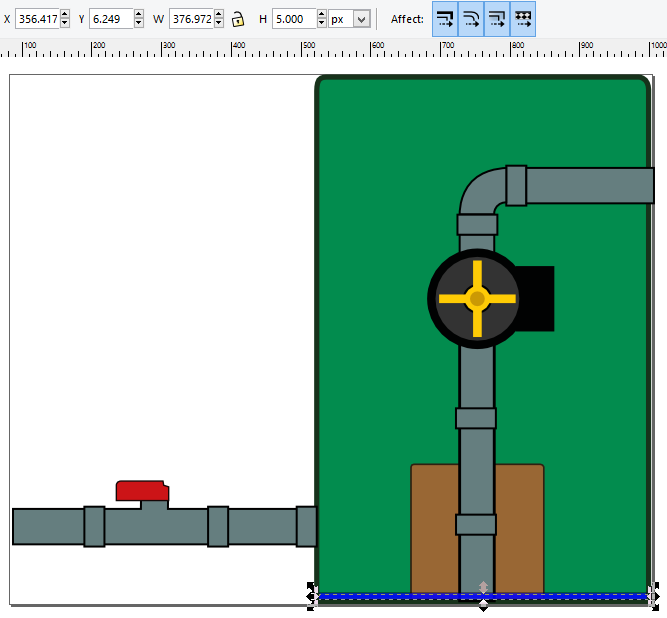
\includegraphics [height=6.5cm]  {obrazky/obr6.png}
		\caption{Prázdna nádrž prečerpávacej stanice}
		\label{picture6}
	\end{center}
\end{figure}


\subsection{Plná nádrž}
Na obrázku č. \ref{picture5} je vykreslená plná nádrž. Hladina má súradnice x, a šírku rovnakú ako v prázdnej nádrži. Zmenila sa os y, a výška - na 1320,16 a na 605,92. 

\begin{figure}[hp]
	\begin{center}
		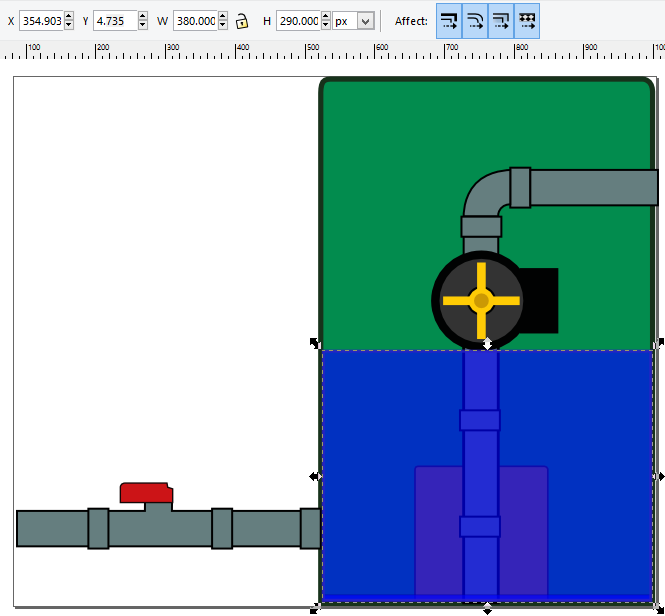
\includegraphics [height=6.5cm]  {obrazky/obr5.png}
		\caption{Plná nádrž}
		\label{picture5}
	\end{center}
\end{figure}

V SVG súbore je to zapísané nasledovným kódom. 

\begin{lstlisting} [language=html]
<rect
	inkscape:label="#hladina"
	y="1320.1689"
	x="2507.8459"
	height="605.83868"
	width="797.04492"
	id="hladina"
	style=
		"fill:#0000ff;
		fill-opacity:0.65098039;
		fill-rule:evenodd;
		stroke:#2c20c8;
		stroke-width:7.42523718px;
		stroke-linecap:butt;
		stroke-linejoin:miter;
		stroke-opacity:0.80952382">
</rect>
\end{lstlisting}


Parametre ako stroke, fill, a iné sa dajú meniť prostredníctvom attr v Snap. … TODO

